\documentclass[11pt,a4paper,twoside,openright]{book}
\usepackage{amsmath}
\usepackage{geometry}
\usepackage{fullpage}
\usepackage{pbox}
\usepackage[usenames,dvipsnames]{color}
%\usepackage{amsmath}
\usepackage{graphicx}
\usepackage{float}
\usepackage{booktabs}
\usepackage{multirow}
\usepackage{wrapfig}							% allows wrapping text around figures
%\usepackage{cite}
%\usepackage[labelfont=bf]{caption}
\usepackage{titlesec}
\titleformat{\section}[block]{\large\bfseries}{\thesection}{1em}{}
\usepackage{framed}
\usepackage{multicol}
\usepackage{hyperref}
\usepackage{enumerate}
\usepackage{enumitem}
\usepackage{setspace}

\setlength{\marginparwidth}{0pt}
%\geometry{legalpaper, margin=0.5in}


 % Define commands to assure consistent treatment throughout document
% \newcommand{\eqnref}[1]{(\ref{#1})}
 \newcommand{\class}[1]{\texttt{#1}}
 \newcommand{\package}[1]{\texttt{#1}}
 \newcommand{\file}[1]{\texttt{#1}}
 \newcommand{\BibTeX}{\textsc{Bib}\TeX}
\renewcommand{\thesection}{\arabic{section}.}
\renewcommand{\thesubsection}{{\thesection}\Alph{subsection}.}
\renewcommand{\thesubsubsection}{\alph{subsubsection}.}

\def\beq{\begin{equation}}
\def\eeq{\end{equation}}
\def\beqn{\begin{matrix}}
\def\eeqn{\end{matrix}}

\begin{document}

\begin{center}{\LARGE SOME USEFUL AND NOT SO USEFUL EQUATIONS}\end{center}

\begin{tabular}{|l | l|}
  \hline
  Order of Operations & x = 1/(2+1)=0.333~vs~x=1/2+1=1.5 \\
  \hline
  Format & format long g for 15 significant digits \\
  \hline
  Variable Types & double = 8 bytes , char = 2 bytes \\
  \hline
  Bits to Bytes & 8 bits = 1 byte \\
  \hline
  Base10 to Base2  & bin2dec(), dec2bin() \\
  \hline
  Double to ASCII  & char(), double() \\
  \hline
  Double to Char  & num2str(), str2num() \\
  \hline
  Inputting Vectors & x = [1 2 3 4] \\
  \hline
  Inputting Matrices & x = [1 2; 3 4] \\
  \hline
  Transpose & x = x' \\
  \hline
  {\it start:increment:end} & x = 1:2:10 yields
  [1 3 5 7 9] \\
  \hline
  {\it linspace(start,end,numpts)} & x =
  linspace(1,10,5) yields [1 3.25 5.5 7.75 10] \\
  \hline
  Length Command & length(x) will compute the length of a vector \\
  \hline
  Matrices of Zeros and Ones & zeros(row,col), ones(row,col)
  \\
  \hline
  Dot Operator & u = [1 2 3]; v = [1 2 3]; u.*v = [1 4 9] \\
  \hline
  Matrix multiplication & u = [1 2 3]; v = [1;2;3]; u*v = 14 \\
  \hline
  Reference Elements of an Array & u = [3 8 9]; u(3) is 9 \\
  \hline
  Reference Elements of a Matrix & A = [3 8 ;9 10]; A(2,1) is 9 \\
  \hline
  Reference Entire Row & A = [3 8 ;9 10]; A(:,1) is the first column
  \\
  \hline
  Evaluating Functions & x = linspace(-pi,pi,100); y = sin(x) + 5; \\
  \hline
  Function Headers & function [out1,out2] =
  name\_of\_function(in1,in2) \\
  \hline
  If/Else/End & \pbox{12cm}{if {\it statement} \\{\it execute this block of code if true}  \\  else \\ {\it execute this block of code if false}\\ end} \\
  \hline
  Logical Operators & $==,>=,<=,>,<,\sim=$ \\
  \hline
  Summation with a For loop & \pbox{12cm} {I = 0; \\ for idx =
  1:2:10 \\ I = I + idx; \\ end} \\
  \hline
  Summation with a While Loop & \pbox{12cm}{I = 0; idx = 1;\\while idx $<=$ 10\\I = I+idx;\\idx = idx + 2;\\end}\\
  \hline
  Plotting & x = linspace(-pi,pi,100); y=sin(x); plot(x,y) \\
  \hline
  Meshing & \pbox{12cm}{x = linspace(-pi,pi,100);y =
    linspace(-pi,pi,100);\\ $[$xg,yg] = meshgrid(x,y);zg = sin(xg.*yg);\\mesh(xg,yg,zg)}\\
  \hline
  Parts of the Computers &
  CPU,Motherboard,GPU,RAM,HDD,I/O \\
  \hline
  Absolute Error & $|actual-computed|$ \\
  \hline
  Percent Error & $(Absolute Error)/actual$ \\
  \hline
  Base 10 to Binary & $15_{10} = 8 + 4 + 2 + 1 = 2^3 + 2^2 + 2^1 + 2^0
  = 1111_2$ \\
  \hline
  Binary to Base10 & $110_2 = 1*2^2 + 1*2^1 + 0*2^0 = 4+2 = 6_{10}$\\
  \hline
  Capital Letters to ASCII & $A = 65_{10}, B = 66_{10}, etc$ \\
  \hline
  Lower Letters to ASCII & $a = 97_{10}, b = 98_{10}, etc$ \\
  \hline
  Examples of ASCII & $cat = [99_{10},97_{10},116_{10}] = 1100011_2,1100001_2,1110100_2$\\
  \hline
\end{tabular}

\newpage

\begin{tabular}{|l | l|}
\hline
Taylor Series & $f(t_{i+1}) \approx f(t_i) + f'(t_i)\Delta t +
f''(t_i)\frac{\Delta t^2}{2!} +
... + f^{(N)}(t_i)\frac{\Delta
  t^N}{N!}$\\
\hline
Bi-Section Method & \pbox{12cm}{Define upper(xU) and lower(xL) bounds
  \\ $x_{new} =
  (xU+xL)/2$\\$if~f(x_{new})>0,x_U=x_{new}~else~x_L=x_{new}$}\\
\hline
Newton-Raphson & $x_{i+1} = x_i - \frac{f(x_i)}{f'(x_i)}$\\
\hline
Newton-Raphson (Optimization) & $x_{i+1} = x_i - \frac{f'(x_i)}{f''(x_i)}$\\
\hline
First-Order Forward Differencing & $f'(x_{i}) \approx
\frac{f(x_{i+1})-f(x_i)}{\Delta x}$\\
\hline
First-Order Backward Differencing & $f'(x_{i}) \approx \frac{f(x_{i})-f(x_{i-1})}{\Delta x}$\\
\hline
First-Order Center Differencing & $f'(x_{i}) \approx \frac{f(x_{i+1})-f(x_{i-1})}{2\Delta x}$\\
\hline
First-Order Second Derivative & $f''(x_{i}) \approx \frac{f(x_{i+2}) -2 f(x_{i+1}) + f(x_i)}{\Delta x^2}$\\
\hline
Secant Method & Combine Newton-Raphson with First-Order Derivative \\
\hline
Reimmann Sum &  $x(t) \approx x_0 + \sum\limits_{i=1}^Nv(t_i) \Delta
t$\\
\hline
Trapezoidal Rule & $I \approx \sum\limits_{i=1}^{N}\frac{1}2 (f(t_i)+f(t_i+\Delta t))\Delta t$\\
\hline
Euler's Method &  $f_2 \approx f_1 + \dot{f}_1\Delta t $\\
\hline
Runge-Kutta-4 & $\begin{matrix}
y_{k+1} = y_k + \phi \Delta t~~~\phi = \frac{1} 6(k_1 + 2 k_2 + 2 k_3 + k_4) \\
k_1 = f(t_k,y_k)~~~k_2 = f(t_k + \Delta t/2\\
y_k + k_1 \Delta t/2)~~~k_3 = f(t_k + \Delta t/2,y_k + k_2 \Delta t/2) \\
k_4 = f(t_k + \Delta t,y_k + k_3 \Delta t)~~~\dot{y} = f(t,y)
\end{matrix}$\\
\hline
Determinant & if A = [a b;c d], det(A) = a*d-b*c \\
\hline
Inverse & $[A|I]$ perform rref to yield $[I|A^{-1}]$\\
\hline
Solve for Eigenvalues & det(sI-A) = 0\\
\hline
Solve for Eigenvectors & $(sI-A)\vec{v}=0$\\
\hline
Eigenvalue Decomposition & $A=V\Lambda V^{-1}$\\
\hline
Solution to ODEs & $\vec{x}(t) = a_1\vec{v}_1e^{\lambda_1 t} + \hdots +
     a_N\vec{v}_Ne^{\lambda_N t} = \sum\limits_{n=1}^N a_n\vec{v}_n
     e^{\lambda_n t}$\\
\hline
Alternate Solution to ODEs & $\vec{x}(t) = e^{At}\vec{x}_0$ \\
\hline
Heat Equation & $\frac{d^2 T}{d x^2} - h'(T-T_a) = 0$\\
\hline
FDM (Heat Equation) & $-T_{i-1} + (2+h'\Delta x^2)T_i - T_{i+1} = h'\Delta x^2 T_a$\\
\hline
2-D Heat Equation &  $\frac{\partial^2 T}{\partial x^2} +
\frac{\partial^2 T}{\partial y^2} = 0$\\
\hline
FDM (2-D Heat Eq) & $T_{i+1,j} + T_{i-1,j} + T_{i,j+1} -
4T_{i,j} + T_{i,j-1} = 0$\\
\hline
Time Dependent Heat Eq &  $k\frac{\partial^2 T}{\partial x^2} =
\frac{\partial T}{\partial t}$\\
\hline
FDM (Heat Eq Time) & $T_i^{l+1} = T_i^l + \lambda (T_{i+1}^l - 2T_i^l
+ T_{i-1}^l)$\\
\hline
Crank-Nicolson & $-\lambda T_{i-1}^{l+1} +2(1+\lambda) T_{i}^{l+1} - \lambda
    T_{i+1}^{l+1} = \lambda T_{i-1}^l + 2(1- \lambda)T_{i}^l + \lambda
    T_{i+1}^l$\\
\hline
$\lambda$ & $\frac{k\Delta t}{\Delta x^2}$\\
\hline
Stiffness for a Bar Element & $\left[K_{(e)}\right] =
k\left[ \begin{matrix} 1   &-1   \\  -1  &1 \end{matrix} \right]$\\
\hline
Stiffness for a Bar & $[K] = \sum\limits_{e=1}^n \left[K_{(e)}\right]$\\
\hline
Bar Equation & $[K]\vec{d} = \vec{F}$\\
\hline
FEA Heated Rods & $\frac{1}{x_2-x_1} \begin{bmatrix} 1 & -1 \\ -1 &
  1 \end{bmatrix} \begin{Bmatrix} T_1 \\ T_2 \end{Bmatrix}
= \begin{Bmatrix} -T^{'}_1 \\ T^{'}_2 \end{Bmatrix}
+ \begin{Bmatrix} \int\limits_{x_1}^{x_2} f(x) N_1 dx
  \\ \int\limits_{x_1}^{x_2} f(x) N_2 dx \end{Bmatrix}$\\
\hline
\end{tabular}


%% \subsection{Finite Element Analysis - Heated Rods - Chapter 31}

Let's re-investigate the heat conduction equation we encountered in
the finite difference methods Section \ref{s:heat1D}. The rod is
discretized in the normal fashion into 5 nodes where the endpoint
temperature values are known as shown in the figure below.

\begin{figure}[H]
  \begin{center}
    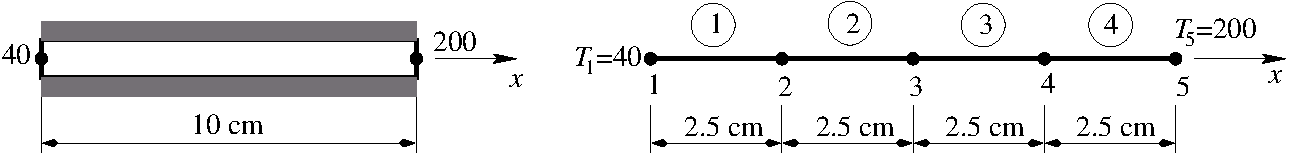
\includegraphics[height=0.1\textwidth,width=0.7\textwidth]{Graphics/L07_F3.pdf}
  \end{center}
\caption{{\bf 1-D Heat Rod for Finite Element Analysis}}\label{f:heatconduction}
\end{figure}

If the body obey's Fourier's law 

\begin{equation}
q = -k \frac{dT}{dx}
\end{equation}

If $k$ is a constant

\beq
k\frac{d^2T}{dx^2} + Q(x) = 0
\eeq

where $Q(x)=dq(x)/dx$ is an internal uniform heat source. 

\begin{enumerate}

\item {\bf Analytic Solution with Q(x) = 0}

The easiest finite element solution is the direct method as has been
done with bars and trusses. This method only applies to $Q(x)=0$. such that 

\beq
\frac{d^2T}{dx^2} = 0
\eeq

To solve the equation the equation above is integrated twice to yield

\beq
T(x) = c_1 x + c_2
\eeq

The boundary conditions are then used to solve for the coefficients
$c_1$ and $c_2$. 

\beq
\begin{matrix}
T(x=0) = T_1 = c_2 = 40 \\
T(x=10) = T_2 = c_1 (10) + 40 = 200 \rightarrow c_1 = 16
\end{matrix}
\eeq

Thus the analytical solution is 

\beq\label{e:heat_rod_direct}
T(x) = 16x+40
\eeq

\item {\bf Direct Method Solution}

Although this equation can be solved for explicitly it is a good
problem to do for its simplicity. Again the question is
to determine the temperature at the nodes in the rod. First let's
examine one element where

\beq\label{e:weighted}
T(x) = N_1T_1 + N_2T_2
\eeq

In this fashion

\beq
\frac{dT}{dx} = T^{'} = \frac{T_2-T_1}{x_2-x_1}
\eeq

which was derived in the previous section. This leads to the heat flux
at node 1 equal to the following.

\beq
q_1 = -k\frac{T_2-T_1}{x_2-x_1} = -kT^{'}
\eeq

In the finite element bar example subject to an axial load, the forces applied
to the beam are equal and opposite. Here similar constraints are
imposed such that $q_1 = -q_2$. This implies that the heat flux
flowing out of 1 bar is equal to the heat flux flowing into 2. Thus,

\beq
q_2 = kT^{'} = k\frac{T_2-T_1}{x_2-x_1}
\eeq

Writing this in matrix form yields the element matrix equation  

\beq
\frac{-k}{x_2-x_1} \begin{bmatrix} -1 & 1 \\ 1 &
  -1 \end{bmatrix} \begin{Bmatrix} T_1 \\ T_2 \end{Bmatrix}
= k \begin{Bmatrix} -T^{'} \\ T^{'} \end{Bmatrix}
\eeq

Dividing out the thermal coefficient $k$, distributing the minus sign
and noting that $T^{'}$ at node 1 is $T^{'}=T^{'}_1$ and $T^{'}=T^{'}_2$ at
node 2 yields the following element matrix.

\beq\label{e:fea_rod_matrix}
\frac{1}{x_2-x_1} \begin{bmatrix} 1 & -1 \\ -1 &
  1 \end{bmatrix} \begin{Bmatrix} T_1 \\ T_2 \end{Bmatrix}
= \begin{Bmatrix} -T^{'}_1 \\ T^{'}_2 \end{Bmatrix}
\eeq

At this point the solution is the same as a bar subject to axial
loads. 

\item {\bf Heat Conduction Bar Example}

Let's now solve the heat conduction problem for the rod in Figure
\ref{f:heatconduction}. First let's write the element stiffness matrix
for elements 1-4. Note that there are 5 nodes and 4 elements where
$x_2-x_1 = \Delta x = 2.5$.

\beq
\begin{bmatrix} 0.4 & -0.4 \\ -0.4 &
  0.4 \end{bmatrix} \begin{Bmatrix} 40 \\ T_2 \end{Bmatrix}
= \begin{Bmatrix} -T^{'}_1 \\ T^{'}_2 \end{Bmatrix}
\eeq

\beq
 \begin{bmatrix} 0.4 & -0.4 \\ -0.4 &
  0.4 \end{bmatrix} \begin{Bmatrix} T_2 \\ T_3 \end{Bmatrix}
= \begin{Bmatrix} -T^{'}_2 \\ T^{'}_3 \end{Bmatrix}
\eeq

\beq
\begin{bmatrix} 0.4 & -0.4 \\ -0.4 &
  0.4 \end{bmatrix} \begin{Bmatrix} T_3 \\ T_4 \end{Bmatrix}
= \begin{Bmatrix} -T^{'}_3 \\ T^{'}_4 \end{Bmatrix}
\eeq

\beq
 \begin{bmatrix} 0.4 & -0.4 \\ -0.4 &
 0.4 \end{bmatrix} \begin{Bmatrix} T_4 \\ 200 \end{Bmatrix}
= \begin{Bmatrix} -T^{'}_4 \\ T^{'}_5 \end{Bmatrix}
\eeq

Just as before this is combined to a full bar element matrix such that

\beq\label{e:fea_rod_matrix_solution}
\begin{bmatrix} 0.4 & -0.4 & 0 & 0 & 0 \\
-0.4 & 0.8 & -0.4 & 0 & 0 \\
0 & -0.4 & 0.8 & -0.4 & 0 \\
0 & 0 & -0.4 & 0.8 & -0.4 \\
0 & 0 & 0 & -0.4 & 0.4 \end{bmatrix}\begin{Bmatrix} 40
  \\ T_2 \\ T_3 \\ T_4 \\ 200 \end{Bmatrix} = \begin{Bmatrix} -T_1^{'}
  \\ 0 \\ 0\\0\\T_5^{'}\end{Bmatrix}
\eeq

Notice that the internal heat flux was canceled due to equal and
opposite reactions. The formulation of these equations led to two
unknowns being introduced. That is, $T_1^{'}$ and $T_5^{'}$ are now
unknowns. The equations must be rearranged to yield the following
equations. 

\beq
\begin{bmatrix} 1 & -0.4 & 0 & 0 & 0 \\
0 & 0.8 & -0.4 & 0 & 0 \\
0 & -0.4 & 0.8 & -0.4 & 0 \\
0 & 0 & -0.4 & 0.8 & 0 \\
0 & 0 & 0 & -0.4 & -1 \end{bmatrix}\begin{Bmatrix} T_1^{'}
  \\ T_2 \\ T_3 \\ T_4 \\ T_5^{'} \end{Bmatrix} = \begin{Bmatrix} -16
  \\ 16 \\ 0\\80\\-80\end{Bmatrix}
\eeq

This equation is of the form $A\vec{x} = \vec{b}$ which can be solved
explicitly for the temperature. The figure below shows the result of
the analytic solution from equation \ref{e:heat_rod_direct} and the
numerical solution from above.

\begin{figure}[H]
  \begin{center}
    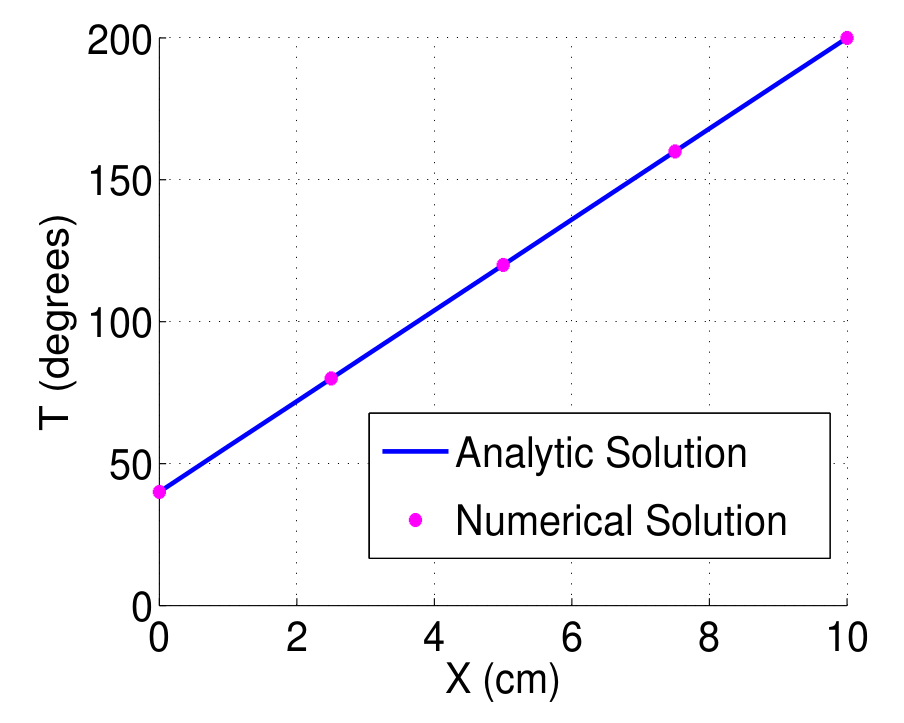
\includegraphics[height=0.4\textwidth,width=0.5\textwidth]{Graphics/Heat_Rod_Direct}
  \end{center}
\end{figure}

\item {\bf Method of Weighted Residuals}

The direct method above works well if $Q(x) = 0$; however, it is it's
major shortcoming. Let's re-investigate the same problem above however
setting $Q(x)/k = 10$. This equation can again be solved analytically
since

\beq
\frac{d^2T}{dx^2} = -10
\eeq

which leads to the temperature solution shown below where the boundary
conditions $T(0) = 40$ and $T(10) = 200$ are used to solve for the
undetermined coefficients. 

\beq
T(x) = -5 x^2 + 66 x + 40
\eeq

In order to solve this using finite element analysis the heat equation
is written as

\beq
\frac{d^2T}{dx^2} + f(x) = 0
\eeq

Then using equation \ref{e:weighted} which is an approximate solution
leads to 

\beq
\frac{d^2\tilde{T}}{dx^2} + f(x) = R
\eeq

where R is a residual since the equation is only an approximation. The
method of weighted residuals then requires

\beq
\int\limits_D R W_i dD = 0
\eeq

where $W_i$ are weights force the integrand to zero. D is the entire
control volume. For this case the control volume is the length of the
rod and the weighted functions are the interpolation functions
$N_i$. This method is called Galerkin's method.

\beq
\int\limits_D R N_i dD = 0 = \int\limits_{x_1}^{x_2}
\left[\frac{d^2\tilde{T}}{dx^2} + f(x)\right] N_i~dx = 0
\eeq

which can also be written as

\beq\label{e:mwr1}
\int\limits_{x_1}^{x_2}\frac{d^2\tilde{T}}{dx^2}N_i~dx= -\int\limits_{x_1}^{x_2} f(x) N_i dx
\eeq

The integrand on the left can be evaluated using integration by parts

\beq\label{e:mwr2}
\int\limits_{x_1}^{x_2}\frac{d^2\tilde{T}}{dx^2}N_i~dx = N_i \frac{d\tilde{T}}{dx} \Big|_{x_1}^{x_2}-\int\limits_{x_1}^{x_2}\frac{d\tilde{T}}{dx}\frac{dN_i}{dx}dx
\eeq

The first term on the right hand side can be evaluated to yield 

\beq\label{e:mwr3}
N_1 \frac{d\tilde{T}}{dx} \Big|_{x_1}^{x_2} =
N_1(x_2)T_2^{'} - N_1(x_1)T_1^{'}
\eeq

where $i=1$. Remember that $N_1(x_2)=0$ and $N_1(x_1)=1$ so

\beq
N_1 \frac{d\tilde{T}}{dx} \Big|_{x_1}^{x_2} = -T_1^{'}
\eeq

Similarly with $i=2$ 

\beq
N_2 \frac{d\tilde{T}}{dx} \Big|_{x_1}^{x_2} = T_2^{'}
\eeq

using equations \ref{e:mwr1} through \ref{e:mwr3} leads to the
following two equations for $i=1$ and $i=2$ 

\beq
\int\limits_{x_1}^{x_2}\frac{d\tilde{T}}{dx}\frac{dN_1}{dx}dx =
-T_1^{'} + \int\limits_{x_1}^{x_2} f(x) N_1 dx
\eeq

\beq
\int\limits_{x_1}^{x_2}\frac{d\tilde{T}}{dx}\frac{dN_2}{dx}dx =
T_2^{'} + \int\limits_{x_1}^{x_2} f(x) N_2 dx
\eeq

The first terms in the left-hand side are simple to evaluate using the
shape functions. 

\beq
\int\limits_{x_1}^{x_2}\frac{d\tilde{T}}{dx}\frac{dN_1}{dx}dx = -\frac{T_2-T_1}{x_2-x_1}
\eeq

\beq
\int\limits_{x_1}^{x_2}\frac{d\tilde{T}}{dx}\frac{dN_2}{dx}dx = \frac{T_2-T_1}{x_2-x_1}
\eeq

If the equation above is written in matrix form the equation is
identical to the element matrix written in \ref{e:fea_rod_matrix}
except there is an external forcing function added that must be
evaluated. 

\beq
\frac{1}{x_2-x_1} \begin{bmatrix} 1 & -1 \\ -1 &
  1 \end{bmatrix} \begin{Bmatrix} T_1 \\ T_2 \end{Bmatrix}
= \begin{Bmatrix} -T^{'}_1 \\ T^{'}_2 \end{Bmatrix}
+ \begin{Bmatrix} \int\limits_{x_1}^{x_2} f(x) N_1 dx
  \\ \int\limits_{x_1}^{x_2} f(x) N_2 dx \end{Bmatrix}
\eeq

The solution to the example with $Q(x)/L = 10$ is solved in the same
fashion as before only the forcing functions must be evaluated for
each element. Just as before this is done for all 4 elements to yield
8 equations. The equations are then stacked together to yield only 5
equations as shown in the equations below. The equations are again
identical to \ref{e:fea_rod_matrix_solution} only the forcing function
adds a bit extra to the equation.

\beq
\begin{bmatrix} 0.4 & -0.4 & 0 & 0 & 0 \\
-0.4 & 0.8 & -0.4 & 0 & 0 \\
0 & -0.4 & 0.8 & -0.4 & 0 \\
0 & 0 & -0.4 & 0.8 & -0.4 \\
0 & 0 & 0 & -0.4 & 0.4 \end{bmatrix}\begin{Bmatrix} 40
  \\ T_2 \\ T_3 \\ T_4 \\ 200 \end{Bmatrix} = \begin{Bmatrix} -T_1^{'}
  + 12.5
  \\ 25 \\ 25 \\ 25 \\ T_5^{'} + 12.5 \end{Bmatrix}
\eeq

Just as before the equations are altered to solve for the introduced
unknowns $T_1^{'}$ and $T_2^{'}$ which leads to the equation

\beq
\begin{bmatrix} 1 & -0.4 & 0 & 0 & 0 \\
0 & 0.8 & -0.4 & 0 & 0 \\
0 & -0.4 & 0.8 & -0.4 & 0 \\
0 & 0 & -0.4 & 0.8 & 0 \\
0 & 0 & 0 & -0.4 & 1 \end{bmatrix}\begin{Bmatrix} T_1^{'}
  \\ T_2 \\ T_3 \\ T_4 \\ T_5^{'} \end{Bmatrix} = \begin{Bmatrix} -3.5
  \\ 41 \\ 25 \\ 105 \\ -67.5 \end{Bmatrix}
\eeq

Again, this can be solved on any numerical computer and the solution
is shown in the figure below.

\begin{figure}[H]
  \begin{center}
    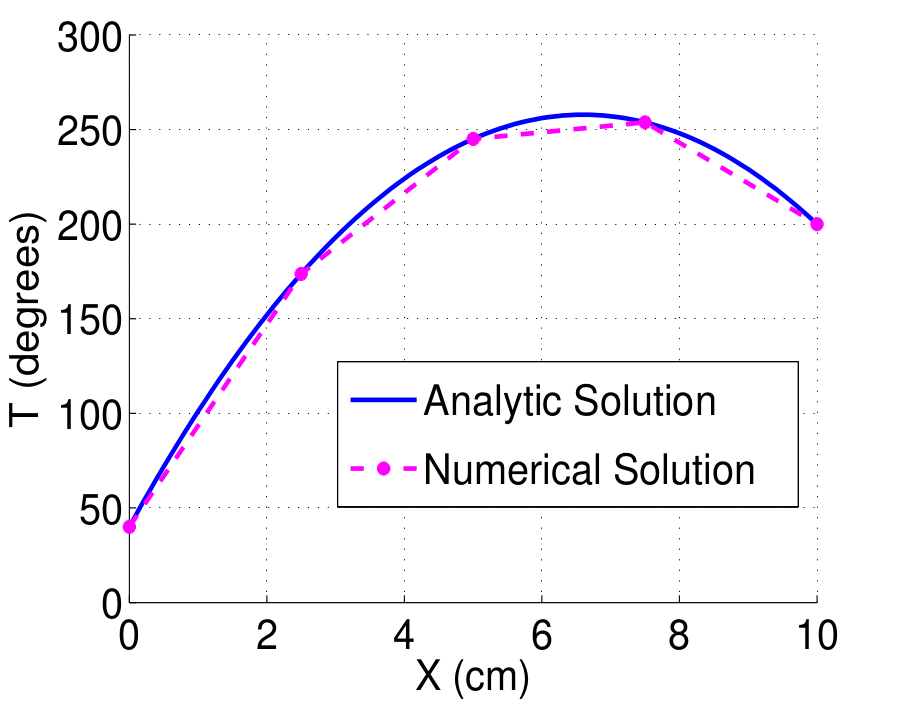
\includegraphics[height=0.4\textwidth,width=0.5\textwidth]{Graphics/Heat_Rod_FEA}
  \end{center}
\end{figure}

Notice however that the solution is not quite exact since the shape
functions are linear. Obviously there are solutions where the shape
functions are quadratic but these are beyond the scope of this text.

\end{enumerate}
    




%% \subsection{Least Squares Regression - Chapter 17}\label{s:lsr}

\begin{enumerate}

\item {\bf Linear Regression}

Linear Regression attempts to fit a line to a function $f$ such that

\begin{equation}
y = f(x) \approx a_0 + a_1 x
\end{equation}

The solution of the coefficients $a_0$ and $a_1$ are found by
minimizing the square error between the actual value of y and the estimated
value. That is,

\begin{equation}
min[\sum\limits_{i=0}^N (y_i - a_0 - a_1 x_i)^2]
\end{equation}

The easiest way to solve this is by using gaussian elimination. First
let $Y$ be a vector of all actual values $y_i$, X be a vector of all
actual values $x_i$ and let $A = [a_0~a_1]^T$.

\begin{equation}
Y = [1~X] A
\end{equation}

We can then say that $H = [1~X]$. The problem above has been solved by
Gauss. The idea is to obtain the least squares estimate of A using the
form $Y=HA$. The solution is

\begin{equation}
A^* = (H^TH)^{-1}H^TY
\end{equation}

Notice how A has been replaced with $A^*$ this is because $H^TH$ is a
2x2 matrix. The problem has been reduced from a system of N points to
a 2x2 system and thus information has been lost because the order of
the system has been truncated. 

\item {\bf Polynomial Regression}

The benefit of using the formula above is that it can be extended to
include polynomials. That is assume we are trying to fit 

\begin{equation}
y \approx a_0 + a_1 x + a_2 x^2 + ... a_n x^N
\end{equation}

Using Gauss' formula we can write

\begin{equation}
Y = [1~X~X^2~...~X^N] A
\end{equation}

where $A = [a_0~a_1~a_2~...~a_N]^T$. Notice that our problem is still
in the form $Y=HA$ and thus we can still use the formula above for
linear regression.

\item {\bf Basis Function Regression}

It is even possible to use the method above to fit a function using
basis functions. For example assume we are trying to fit

\begin{equation}
y \approx a_0 + a_1 f_1(x) + a_2 f_2(x) + ... a_n f_N(x)
\end{equation}

Again this problem can simply be written as 

\begin{equation}
Y = [1~F_1~F_2~...~F_N] A
\end{equation}

and solved just as before.

\item {\bf Goodness of Fit}

Often times it is beneficial to compute the goodness of fit which is a
number that represents how well the regression curve fits the
data. To do this we must first compute the values of y computed by the
regression line. This is very simple once you have computed H, and
$A^*$. 

\begin{equation}
\tilde{Y} = HA^*
\end{equation}

This is equation gives you the y-coordinates as computed by the
regression line. Using this it is possible to compute the total
residuals or the error in the fit and the measured/given data.

\begin{equation}
S_r = \sum\limits_{i=1}^N (Y_i-\tilde{Y}_i)^2
\end{equation}

This value will get bigger when the error between the fit and the data
are large. However, notice that this value changes with the number of
data points. If there are more data points the error can get quite
large which doesn't necessarily help. Instead what we do is compute
the error between the mean of Y which is denoted as $\bar{Y}$.

\begin{equation}
S_t = \sum\limits_{i=1}^N (Y_i-\bar{Y})^2
\end{equation}

and then use $S_r$ and $S_t$ to normalize everything and compute $r$
which is the correlation coefficient.

\begin{equation}
r = \sqrt{\frac{S_t-S_r}{S_t}}
\end{equation}

This number can only assume values between 0 and 1. If the value of r
is 1 then the fit is said to be perfect. If the value of r is 0 the
fit is not good.

\end{enumerate}


%% \subsection{Interpolation - Chapter 18}

\begin{enumerate}

\item {\bf Linear Interpolation}

The simplest form of interpolation is by creating a line in between
points $x_1$ and $x_0$ such that

\begin{equation}
y^* = f(x^*) = f(x_0) + \frac{f(x_1)-f(x_0)}{x_1-x_0}(x^*-x_0)
\end{equation}

\begin{figure}[H]
  \begin{center}
    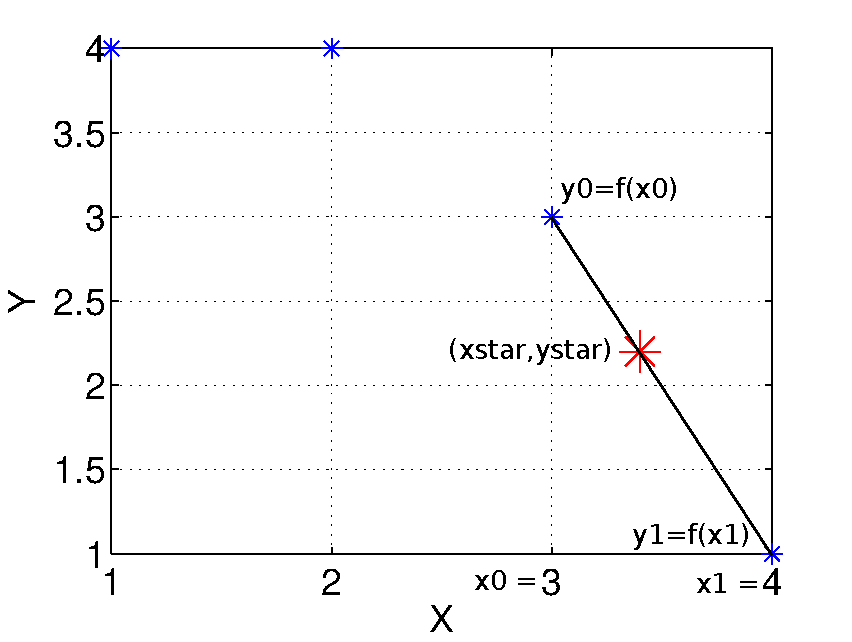
\includegraphics[height=0.5\textwidth,width=0.7\textwidth]{Graphics/Linear_Interpolation.pdf}
  \end{center}
\end{figure}

\item {\bf Polynomial Interpolation}

Note that the problem can be explicitly derived using Linear Regression. That
is we are trying to solve the problem $f(x) = a_0 + a_1(x-x_0)$. If
this problem is set up the solution would yield
$a_0=f(x_0)$ and $a_1$ = {\it slope}. Thus it is possible to extend
the interpolation method to higher order polynomials. Our polynomial
is then

\begin{equation}
\tilde{f}(x) = a_0 + a_1 (x-x_0) + a_2 (x-x_0)^2 + ... a_N (x-x_0)^N
\end{equation}

Note however that in order to interpolate using the equation
above your need N+1 data points. For example, in order to fit a line
the method requires two points to solve for $a_0,a_1$. In order to fit
a quadratic the method requires three points to solve for $a_0,a_1$
and $a_2$.

\begin{figure}[H]
  \begin{center}
    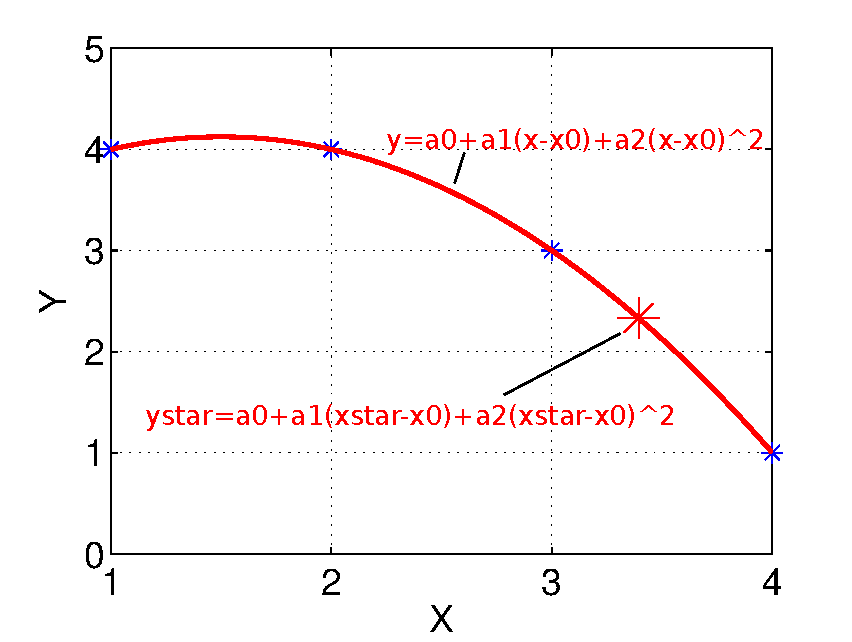
\includegraphics[height=0.5\textwidth,width=0.7\textwidth]{Graphics/Polynomial_Interpolation.pdf}
  \end{center}
\end{figure}

\item {\bf Linear Splines}

Splines are a way to approximate the curve with more than one
model. For example, if you have a curve that looks fourth order you
could fit the entire data set as fourth order polynomial or you could
simply fit the line to 4 linear polynomials. In certain situations
this would actually create a better fit. The equation for linear
splines is simply

\begin{equation}
  \tilde{f}(x) = f(x_{i-1}) + m_{i-1}(x-x_{i-1})~~x_{i-1}\leq x \leq x_i
\end{equation}
where
\begin{equation}
  m_{i-1} = \frac{f(x_{i}) - f(x_{i-1})}{x_{i}-x_{i-1}}
\end{equation}

\item {\bf Quadratic Splines}

The equation for quadratic splines gets a little more messy so the
derivation is left for the student. Instead rules are listed to help
you with the derivation. The basic formula of a quadratic spline is
\begin{equation}
\tilde{f}(x) = a_{i} x^2 + b_{i} x + c_i~~x_{i-1}\leq x \leq x_i
\end{equation}
The rules for quadratic splines are then
\begin{enumerate}
\item The function values of adjacent splines must be equal to each
  other
  \begin{equation}
    a_i x_{i}^2 + b_i x_{i} + c_i = a_{i+1} x_{i}^2 + b_{i+1} x_i + c_{i+1}
  \end{equation}
\item The first and last function must pass through the end points
  \begin{equation}
    \begin{matrix}
      a_1 x_0^2 + b_1 x_0 + c_1 = f(x_0) \\
      a_n x_n^2 + b_n x_n + c_n = f(x_n)
    \end{matrix}
  \end{equation}
\item The first derivative of adjacent splines must be equal to each
  other
  \begin{equation}
    2 a_i x_{i} + b_i = 2 a_{i+1} x_{i} + b_{i+1}
  \end{equation}
\item The second derivative of the first spline at $x_0 = 0$ 
  \begin{equation}
    a_1 = 0
  \end{equation}

\begin{figure}[H]
  \begin{center}
    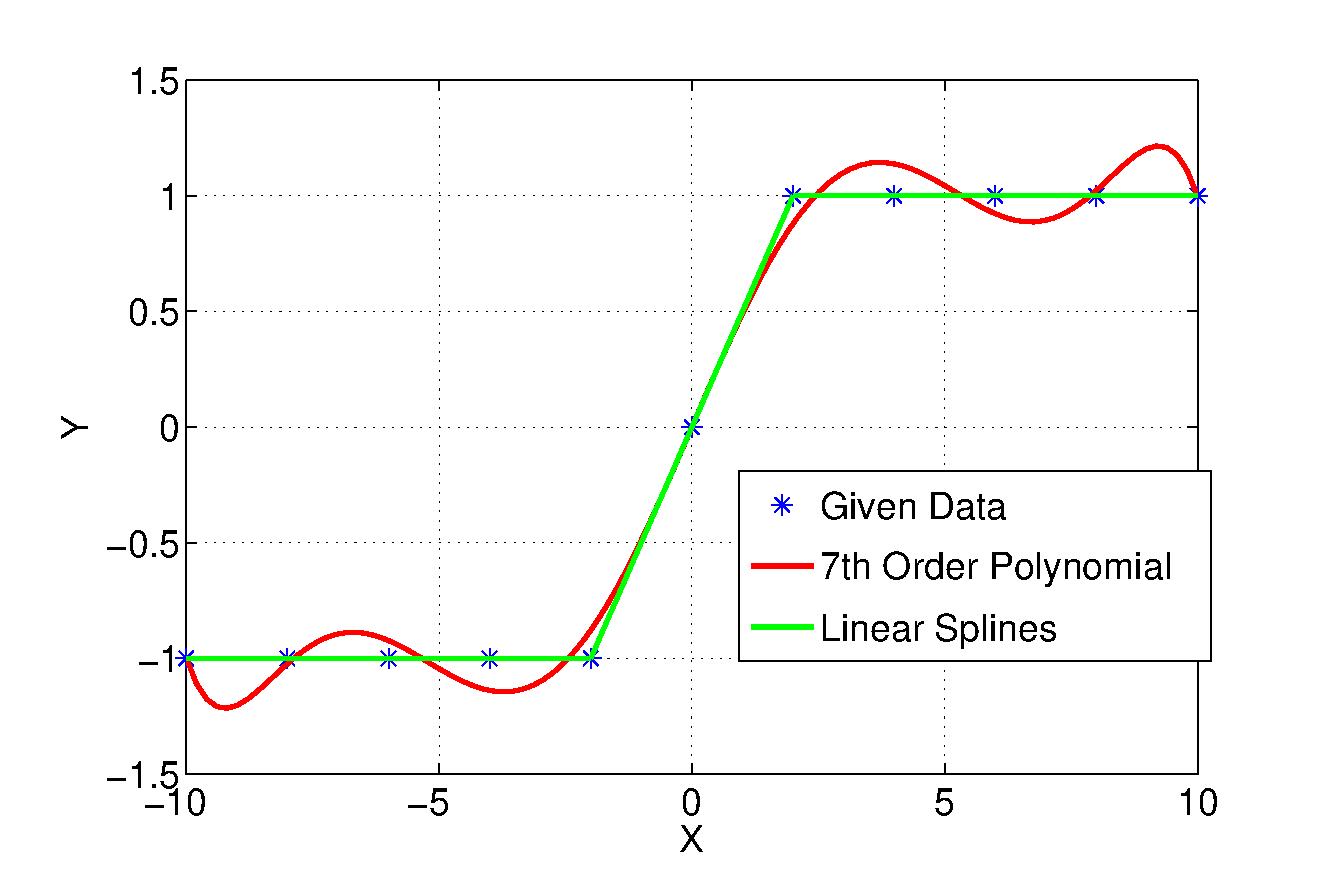
\includegraphics[height=0.5\textwidth,width=0.7\textwidth]{Graphics/Linear_Splines.eps}
  \end{center}
\end{figure}

\clearpage

\begin{figure}[H]
  \begin{center}
    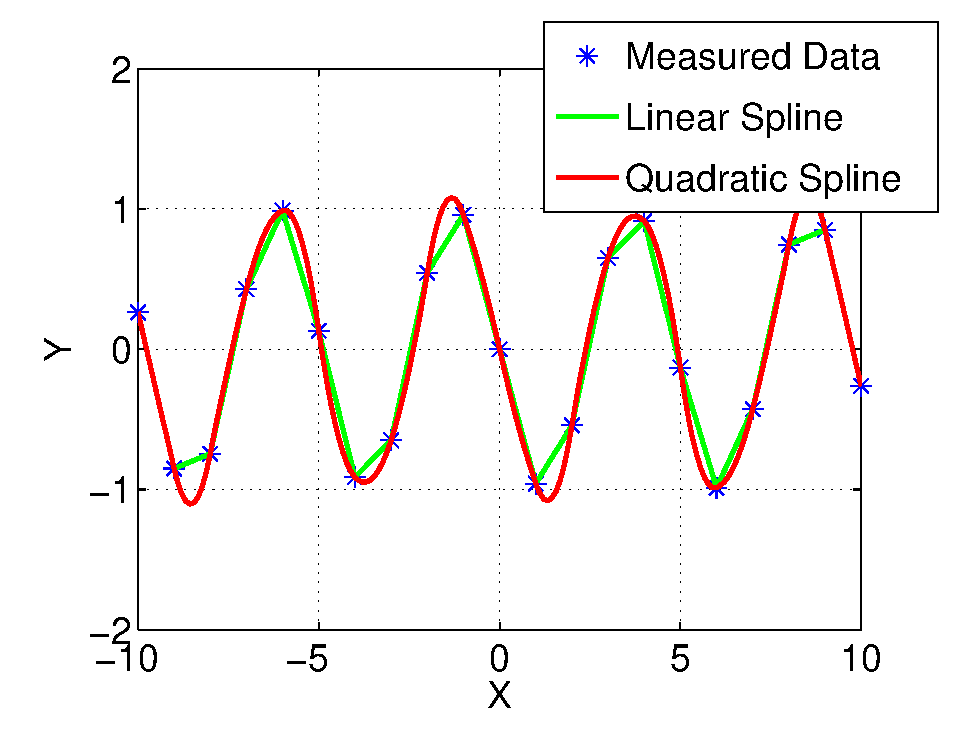
\includegraphics[height=0.5\textwidth,width=0.7\textwidth]{Graphics/Quadratic_Splines.eps}
  \end{center}
\end{figure}

\end{enumerate}

\item {\bf 2-D Interpolation}

It is often the case that rather than your system being of the form
$y=f(x)$ you have an equation of the form $z=f(x,y)$. In this case you
need to use 2-D interpolation and here we will discuss linear 2-D
interpolation called bi-linear interpolation for short. This
interpolation scheme is three separate interpolations. Assume you are
trying to interpolate $z^*=\tilde{f}(x^*,y^*)$ where $x_{i-1}\leq x^*
\leq x_i$ and $y_{i-1}\leq y^* \leq y_i$. The equations to solve for
$z^*$ is then

\begin{equation}
z_U = f(x_{i-1},y_{i}) + \frac{f(x_i,y_i)-f(x_{i-1},y_i)}{x_{i}-x_{i-1}}(x^*-x_{i-1})
\end{equation}
\begin{equation}
z_L = f(x_{i-1},y_{i-1}) + \frac{f(x_i,y_{i-1})-f(x_{i-1},y_{i-1})}{x_{i}-x_{i-1}}(x^*-x_{i-1})
\end{equation}
\begin{equation}
z^* = z_L + \frac{z_U-z_L}{y_i-y_{i-1}}(y^*-y_{i-1})
\end{equation}

The basic solution is simply three linear interpolations to get your
solution.

\begin{figure}[H]
  \begin{center}
    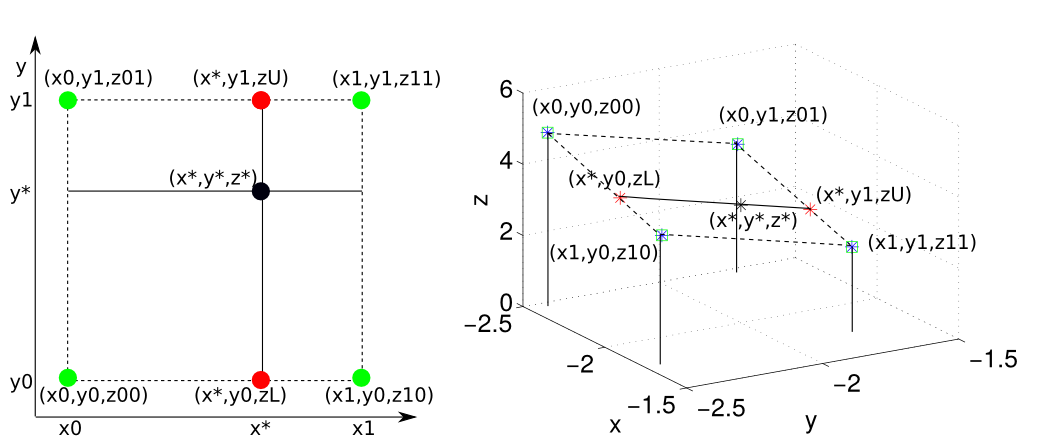
\includegraphics[height=0.4\textwidth,width=0.9\textwidth]{Graphics/TwoD_Interpolation.png}
  \end{center}
\end{figure}

\end{enumerate}



\end{document}
